%=========================================================
% Interrupts and INTC 
%=========================================================
\section{Interrupts and INTC (Interrupt Controller)}

The mmRISC-1 supports the following four interrupt request inputs. 

\begin{description}
    \item[IRQ\_EXT] External Interrupt
    \item[IRQ\_MSOFT] Machine Software Interrupt IRQ\_MTIME Machine Timer Interrupt
    \item[{IRQ[63:0]}] Interrupt Request (towards Interrupt Controller)
\end{description}

Priority among above interrupts is defined as IRQ\_EXT > IRQ\_SOFT > IRQ\_MTIME > IRQ[63:0].
64 IRQ inputs are controlled by INTC (Interrupt Controller) shown in Figure \ref{fig:INTERRUPTS_INTC}. The INTC can be configured by dedicated CSRs. INTCFGSENSE0/1 select each IRQ sense way from level sense or rising edge sense. INTPENDING0/1 show each IRQ input logic level for level sense, or pending status for rising edge sense. For rising edge IRQ, pending status can be cleared by writing 1 to each corresponding bit. INTCFGENABLE0/1 enable or disable each interrupt.\\

INTCFGPRIORITY0/1/2/3 configure priority level of each IRQ. The priority level is expressed in 4bits, 4’b0000 is lowest and 4’b1111 is highest. In priority tournament block, one IRQ having the highest priority level is selected from requesting IRQ, and finally if the priority is larger than MINTCURLVL, the selected IRQ is outputted. When CPU accepts the IRQ request, MINTCURLVL is automatically transferred to MINTPRELVL, and priority level of accepted IRQ is also automatically transferred to MINTCURLVL. In last phase of interrupt software handler before MRET, software should copy MINTPRELVL to MINTCURLVL. Thus IRQ allows nested interrupts.

\begin{figure}[H]
    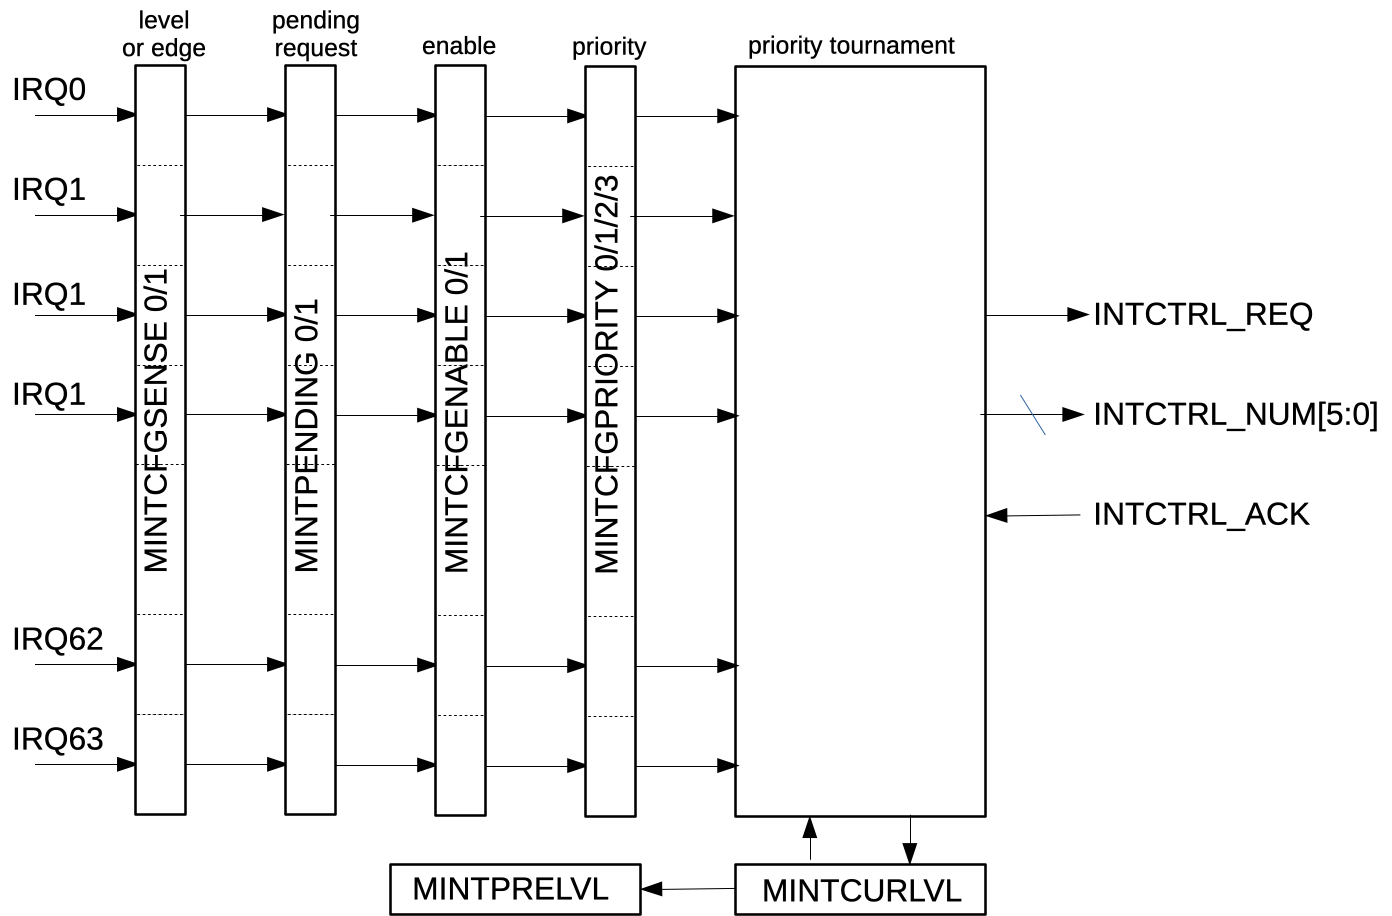
\includegraphics[width=1.00\columnwidth]{./Figure/Interrupts_INTC.png}
    \caption{INTC (Interrupt Controller)}
    \label{fig:INTERRUPTS_INTC}
\end{figure}

An example of a startup routine that includes an exception handler and an interrupt handler is shown in Listing \ref{list:STARTUPROUTINE}. Note that the sample routine ignores saving and restoring Floating Point Registers FRx. Also, an example of an interrupt initialization routine and an interrupt handler routine in the C language portion, which are combined with the startup routine, are shown in Listing \ref{list:INTERRUPTCROUTINE}. In this example, multiple interrupts with different priorities are gathered into one entry point and one handler routine. This example increases the interrupt latency due to the conditional judgment in the handler routine. If you want to improve the latency of an interrupt, it is recommended to prepare a dedicated entry point and handler routine for the interrupt.
%-------------------
\begin{lstlisting}[caption=An Example of Startup Routine including Exception Handlers and Interrupt Handlers, captionpos=b, language=, frame=single, basicstyle=\ttfamily\scriptsize, label=list:STARTUPROUTINE]
_reset:
    j    _start
_vector_base:
    j    _trap_exception // 00:Exception
    j    _trap_illegal   // 01:Reserved
    j    _trap_illegal   // 02:Reserved
    j    _trap_int_soft  // 03:IRQ_MSOFT
    j    _trap_illegal   // 04:Reserved
    j    _trap_illegal   // 05:Reserved
    j    _trap_illegal   // 06:Reserved
    j    _trap_int_timer // 07:IRQ_MTIME
    j    _trap_illegal   // 08:Reserved
    j    _trap_illegal   // 09:Reserved
    j    _trap_illegal   // 10:Reserved
    j    _trap_int_ext   // 11:IRQ_EXT
    j    _trap_illegal   // 12:Reserved
    j    _trap_illegal   // 13:Reserved
    j    _trap_illegal   // 14:Reserved
    j    _trap_illegal   // 15:Reserved
    j    _trap_irq       // 16:IRQ00
    j    _trap_irq       // 16:IRQ01
    j    _trap_irq       // 16:IRQ02
    j    _trap_irq       // 16:IRQ03
    ...
    j    _trap_irq       // 16:IRQ63
//
_trap_exception:
    csrrw x1, mscratch, x1  // swap ra and macratch
    jal   _trap_handler_save
    jal   _trap_handler_exception
    jal   _trap_handler_load
    csrrw ra, mscratch, ra  // swap ra and macratch
    mret
//
_trap_int_soft:
    csrrw ra, mscratch, ra  // swap ra and macratch
    jal   _trap_handler_save
    jal   _trap_handler_int_soft
    jal   _trap_handler_load
    csrrw ra, mscratch, ra  // swap ra and macratch
    mret
//
_trap_int_timer:
    csrrw ra, mscratch, ra  // swap ra and macratch
    jal   _trap_handler_save
    call  INT_Timer_Handler
    jal   _trap_handler_load
    csrrw ra, mscratch, ra  // swap ra and macratch
    mret
//
_trap_int_ext:
    csrrw ra, mscratch, ra  // swap ra and macratch
    jal   _trap_handler_save
    jal   _trap_handler_int_ext
    jal   _trap_handler_load
    csrrw ra, mscratch, ra  // swap ra and macratch
    mret
//
_trap_irq:
    csrrw ra, mscratch, ra  // swap ra and macratch
    jal   _trap_handler_save
    jal   _trap_handler_irq
    jal   _trap_handler_load
    csrrw ra, mscratch, ra  // swap ra and macratch
    mret
//
_trap_illegal:
   j     .
//
_trap_handler_save:
    csrrw ra, mscratch, ra  // swap ra and macratch
    addi  sp, sp, -124
    sw    x1,    0(sp) // ra
    sw    x2,    4(sp) // sp
    sw    x3,    8(sp)
    sw    x4,   12(sp)
    ...
    sw    x30, 116(sp)
    sw    x31, 120(sp)
    csrrw ra, mscratch, ra  // swap ra and macratch
    ret
//
_trap_handler_load:
    csrrw ra, mscratch, ra  // swap ra and macratch
    lw    x1,    0(sp) // ra
    lw    x2,    4(sp) // sp
    lw    x3,    8(sp)
    lw    x4,   12(sp)
    ...
    lw    x30, 116(sp)
    lw    x31, 120(sp)
    addi  sp, sp, 124
    csrrw ra, mscratch, ra  // swap ra and macratch
    ret
//
_trap_handler_exception:
    // As well as _trap_handler_irq
    ret
//
_trap_handler_int_soft:
    // As well as _trap_handler_irq
    ret
//
_trap_handler_int_timer:
    // As well as _trap_handler_irq
    ret
//
_trap_handler_int_ext:
    // As well as _trap_handler_irq
    ret
//
_trap_handler_irq:
    // save PC, MSTATUS,mintprelvl
    csrr  x8, mepc
    csrr  x9, mstatus
    csrr  x10, 0xbf1 //mintprelvl
    addi  sp, sp, -16
    sw    x1 , 0(sp)
    sw    x8 , 4(sp)
    sw    x9 , 8(sp)
    sw    x10,12(sp)
    // enable global interrupt (set mie)
    csrrsi x15, mstatus, 0x08
    // allow enested interrupt
    call   INT_IRQ_Handler         // Defined in C Program
    // disable global interrupt (clear mie)
    csrrci x15, mstatus, 0x08
    // load MSTATUS, PC, mintcurlvl
    lw    x1 , 0(sp)
    lw    x8 , 4(sp)
    lw    x9 , 8(sp)
    lw    x10,12(sp)
    addi  sp, sp, 16
    csrw  0xbf0, x10 // mintcurlvl
    csrw  mstatus, x9
    csrw  mepc, x8
    // Return
    ret
//
// Start Up Routine
//
_start:
    //
    // Init GP and SP
    la  gp, __GLOBAL_PTR__
    la  sp, __STACK_TOP__
    //
    // Copy Initial Data
    la  a0, __ROM_INIT_BGN__  // Defined in Linker Script
    la  a1, __RAM_INIT_BGN__  // Defined in Linker Script
    la  a2, __RAM_INIT_END__  // Defined in Linker Script
    bgeu a1, a2, 2f
1:
    lw t0, (a0)
    sw t0, (a1)
    addi a0, a0, 4
    addi a1, a1, 4
    bltu a1, a2, 1b
2:
    //
    // Clear BSS
    la a0, __BSS_BGN__
    la a1, __BSS_END__
    bgeu a0, a1, 2f
1:
    sw zero, (a0)
    addi a0, a0, 4
    bltu a0, a1, 1b
2:
    //
    // Setup MTVEC
    la   t0, _vector_base
    ori  t0, t0, 0x01 // vectored
    csrw mtvec, t0
    //
    // Goto Main
    call main
    //
    // Forever Loop
3:
    j    3    
\end{lstlisting}
%------------------------------------------
\begin{lstlisting}[caption=An Example of Interrupt Initialization and An Interrupt Handler in the C language portion, captionpos=b, language=, frame=single, basicstyle=\ttfamily\scriptsize, label=list:INTERRUPTCROUTINE]
//--------------------------
// Interrupt Initialization
//--------------------------
void INT_Init(void)
{
    // Configure Interrupt Controller
    write_csr(MINTCFGPRIORITY0, 0x........);
    write_csr(MINTCURLVL      , 0x........);
    write_csr(MINTCFGSENSE0   , 0x........);
    write_csr(MINTCFGENABLE0  , 0x........);
    ....
    // Enable Interrupt
    write_csr(MIE, read_csr(MIE) | (1<<7)); // MTIME Interrupt
    write_csr(MSTATUS, read_csr(MSTATUS) | (1<<3)); // MIE
}

//-------------------------
// Interrupt Handler IRQ
//-------------------------
void INT_IRQ_Handler(void)
{
    uint32_t irq_pend0, ...;
    uint32_t irq_level;
    //
    irq_pend0 = read_csr(MINTPENDING0);
    ...
    irq_level = read_csr(MINTCURLVL);
    //
    // Dispatch
    switch(irq_level)
    {
        // Group Priority Level 1
        case 1 :
        {
            if (irq_pend0 & 0x........)
            {
                Interrput_Handler_for_each_Peripheral();
            }
            break;
        }
        // Group Priority Level 2
        case 2 :
        {
            // ...
            break;
        }
        // ...
        // ...
        // Group Priority Level 15
        case 15 :
        {
            // ...
            break;
        }
    }
}
\end{lstlisting}
